\documentclass[11pt]{article}
\usepackage{amsmath, amscd, amssymb, amsthm}
% \usepackage{diagrams}
\usepackage{color}
\usepackage{graphicx, psfrag, tikz}
\usepackage[all]{xy}
\usepackage[margin=1.1in]{geometry}

\usepackage{enumitem,kantlipsum}
\usetikzlibrary{arrows.meta}
\usetikzlibrary{calc,patterns,angles,quotes}
%\renewcommand{\baselinestretch}{1.17}
\usepackage{chemformula}

\newtheorem{theorem}{Theorem}[section]
\newtheorem{lemma}[theorem]{Lemma} 
\newtheorem{proposition}[theorem]{Proposition}
\newtheorem{corollary}[theorem]{Corollary}
\theoremstyle{definition} 
\newtheorem{definition}[theorem]{Definition}
\newtheorem{conjecture}[theorem]{Conjecture}
\newtheorem{remark}[theorem]{Remark}
\newtheorem{example}[theorem]{Example}

\begin{document}
\begin{center}
\textbf{Math 309 Homework 2}\\
(7 problems)
\end{center}
\vspace{0.2in}


\noindent  \textbf{Reminder:} Solutions should be presented using complete sentences, with grammatically correct English, that combine both words and precise mathematical expressions to articulate your line of reasoning.  Collaboration on homework is encouraged, but you need to write up the solutions in your own words that reflect your own understanding of the material. \\

\begin{enumerate}[leftmargin=*]
\item  If you agree to follow the statement of academic integrity:
\begin{itemize}
\item [ ] 
\emph{``as a member of the UW community, I will treat others with kindness and respect, and I will not take unfair advantage of other students''},
\end{itemize}
throughout this entire course, then check the box on Gradescope.  \\

 \item (a) Write $u''+0.5u'+2u=0$ as a system of first order equations.\\
(b) Write  $u''+0.5u'+2u=3\sin t$ as a system of first order equations.\\

\item (a) Write the following system of two first order equations with initial conditions as a single equation, in one variable $x$, of second order:
\[x_1'=x_1-2x_2, \ \ x_1(0)=-1\]
\[x_2'=3x_1-4x_2,\  \ x_2(0)=2,\]
and write down the initial conditions for this 2nd order equation.

(b) The equation you obtained for $x$ in part a) is a homogeneous 2nd order equation with constant coefficients.  Use what you learned about such equations in Math 307 to find the solutions $x(t)$ satisfying that equation and the initial conditions.

(c)  Use your answer for $x$ in part b), and the relationship  between $x$ and $x_1, x_2$ that you established in part a),  to find the solution $x_1, x_2$ for the above system of equations with initial values.

\iffalse
(d) Write the above system of differential equations in the form 
\[
\left[\begin{array}{l} x_1'\\ x_2'\end{array}\right]=A  \left[\begin{array}{l} x_1\\ x_2\end{array}\right],
\]
where $A$ is a $2\times 2$ matrix.  Then find the general solution, $ \left[\begin{array}{l} x_1 \\ x_2 \end{array}\right]$, to this system by finding the eigenvalues and eigenvectors of the coefficient matrix $A$. 

(e) Use the general solution you found in  part d), now find the solution  $ \left[\begin{array}{l} x_1 \\ x_2 \end{array}\right]$ that also satisfies the above initial values. \\
\fi

\item (Linear triatomic molecule) Triatomic molecules are those composed of three atoms.  The schematic diagram below models carbon dioxide, \ch{CO2}, which is a molecule that has a linear geometry, i.e. it is configured so the three atoms lie in a line.  (Note that many triatomic molecules are not linear, e.g. the three atoms  in \ch{H2O} form an angle of about 104.5 degrees.)

The  \ch{CO2} molecule consists of two oxygen atoms, each of mass $M$, and one carbon atom of mass $m$ in the middle.  

The molecule as a whole can translate or rotate in all directions in the 3D space, but here for simplicity we will only consider one directional motions in the direction parallel to the molecule for each atom.   Let $x_1(t), x_2(t), x_3(t)$ be the displacement away from the equilibrium position for each of the three atoms, respectively as labelled in the diagram.  

When $(x_1, x_2, x_3)=(0,0,0)$, the 3 atoms are in equilibrium.  Note that $(0,0,0)$ is not the only equilibrium position since any $(c,c,c)$, where $c$ is a constant, is also an equilibrium position since such a shift moves the entire molecule without changing the relative distances between the atoms.   And our variables $(x_1, x_2, x_3)$ is the displacement from our chosen reference equilibrium position $(0,0,0)$.

\begin{center}
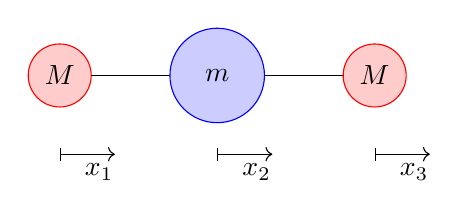
\begin{tikzpicture}
 \draw[red,fill=red!20] (-2, 0) circle (0.4cm);
        \node at (-2, 0) {$M$}; 
  \draw (-1.6,0)--(-0.2,0);     
   \draw[red,fill=red!20] (2, 0) circle (0.4cm);
   \node at (2, 0) {$M$};     
   \draw (0.2,0)--(1.6,0);   
    \draw[blue,fill=blue!20] (0, 0) circle (0.6cm);
   \node at (0, 0) {$m$};     
   
   \draw[|->] (-2,-1) -- (-1.3, -1);
   \node[below] at (-1.5, -1) {$x_1$};
   
    \draw[|->] (0,-1) -- (0.7, -1);
   \node[below] at (0.5, -1) {$x_2$}; 
   
    \draw[|->] (2,-1) -- (2.7, -1);
   \node[below] at (2.5, -1) {$x_3$}; 
     
   \end{tikzpicture}
   \end{center}

Between two atoms, the magnitude of the interatomic force can be a very complicated function $f(r)$ of the distance $r$ between the atoms.  By considering the Taylor expansion of $f(r)$ around $r=r_0$, the equilibrium distance, we have 
\[
f(r)=f(r_0)+ f'(r_0)(r-r_0) + \frac{1}{2}f''(0)(r_0) (r-r_0)^2+\cdots,
\]
where $f(r_0)=0$ since $r_0$ is the equilibrium distance.  We can approximate $f(r)$ by the first term $f(r)\approx f'(r_0)(r-r_0)$ of the Taylor expansion.   In other words, the magnitude of the force between two atoms is approximately a constant multiple of the displacement away from the equilibrium distance between them, which is the same as the coupled spring-mass system we discussed in class.  

(a) Write down a system of differential equations describing the motion of these three atoms.  The first one of the three equations is already given, and you need to finish writing down the other two.  
\[
\begin{array} {cl}
Mx_1'' &= -k(x_1-x_2)\\
mx_2'' & =\\
Mx_3'' & = 
\end{array}.
\]

(b) Write the system of equations from part a) in the form $x''=Fx$, where $x(t)=\left[\begin{array}{l} x_1(t)\\x_2(t)\\ x_3(t)\end{array}\right]$ and $F$ is a $3\times 3$ matrix.  Find the eigenvalues and eigenvectors of the matrix $F$.\\




\item (Hamilton's equations of motion) Newton's equation of motion for a particle of position $x(t)$ subject to a potential $V(x)$ is 
\[
m\frac{d^2x}{dt^2}=-\frac{dV}{dx}(x),
\]
where $m$ is the mass of the particle and $-\frac{dV}{dx}(x)$ is the force due to the potential $V(x)$. When you do this problem, just think of $-\frac{dV}{dx}(x)=F(x)$ as some function of $x$.    

(Note if you've never heard of the word potential before, this concept is perhaps a bit confusing, in which case don't worry about it and just think of it as nothing more than a function.  If you want to get a bit of intuition, think of gravity acting on a falling ball of mass $m$ near the surface of the Earth.  Then $V(x)=mgx$ is a gravitational potential on the ball, where $x$ is the height of the ball, the higher the ball, the larger the potential.  And the force due to gravity is in the direction opposite of the rate of change in this potential, $F=-\frac{dV}{dx}=-mg$.)

Let $p(t)=m\frac{dx}{dt}$ be the moment of the the particle.

(a) Transform Newton's equation of motion above into a system of first order equations by expressing $x'$ and $p'$ as functions of $x$ and $p$,
\[
\begin{cases}
x'=\\
p'=
\end{cases}.
\]
Note the right hand side of the system above needs to be expressed purely as functions of $x$ and $p$, without $x'$ and $p'$.  \\


(b) Let the \emph{Hamiltonian} function be $H(x,p)=\frac{p^2}{2m}+V(x)$ (note that the first term, $\frac{p^2}{2m}$, is the kinetic energy of the particle, so $H$ is the total energy).  

Use your answer from part a) to check that 
\[
\begin{cases}
x'=\frac{\partial H}{\partial p}\\
p'=-\frac{\partial H}{\partial x}
\end{cases}.
\]
This system of equations is known as Hamilton's equations of motion, due to William Rowan Hamilton (1805-1865), and as you have shown above,  it is equivalent to Newton's equation of motion.  Note that this problem is written for $x$ being one dimensional, but it generalizes just as well to when $x=(x_1,\ldots, x_n)^T$ is a vector valued function with almost no notation change besides replacing $\frac{dV}{dx}$ by the gradient $\nabla V(x)=\left(\frac{\partial V(x)}{\partial x_1},\ldots, \frac{\partial V(x)}{\partial x_n}\right)^T$.  Still the whole story is more general than what is explored here since many forces cannot be written as $F(x)=-\nabla V(x)$, e.g. friction and magnetic force.\\

\item (Rolling down an infinite potential hill)  Suppose a particle of mass $m$ is moving in one direction, horizontally,  with its position given by $x(t)$.   Suppose at time $t=0$, the ball is at position $x(0)=0$.

Suppose the particle is subject to a potential given by $V(x)=-\frac{1}{5}x^2$.  The graph of this potential function is shown in the figure below, and it looks like an infinite hill (it continues on outside of the figure).  When $x=0$, the particle is at the very top of this potential hill.  If it moves away from $x=0$, it will experience a drop in the potential.

\begin{center}
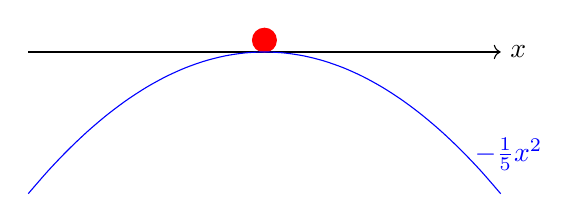
\begin{tikzpicture}
  \draw[->] (-3, 0) -- (3, 0) node[right] {$x$};
   \draw[red,fill=red] (0,0.15) circle (1ex);
   \draw[domain=-3:3, smooth, variable=\x, blue] plot ({\x}, {-0.2*\x*\x});  
   \node at (3.1, -1.3) {\textcolor{blue}{$-\frac{1}{5}x^2$}};
\end{tikzpicture}
\end{center}

(a) Newton's equation for the particle in this potential (c.f. Problem 5) is  
\[
m\frac{d^2x}{dt^2}=-\frac{d}{dx}\left(-\frac{1}{5}x^2\right)=\frac{2}{5}x.
\]
This is a homogeneous 2nd order equation with constant coefficients.  Using what you learned in Math 307 to find the general solution $x(t)$ to this 2nd order equation. Then differentiate $x$ to find $p(t)=m\frac{dx}{dt}$.

(b) Write Newton's equation, $mx''=\frac{2}{5}x$,  
as a system of 1st order equations in $x$ and $p$,
\[
\begin{cases}
x'= \\
p'=
\end{cases}.
\]
After that, write this system in the form of 

\[
\left[\begin{array}{l} x'\\ p' \end{array}\right]=A  \left[\begin{array}{l} x\\ p\end{array}\right],
\]
where $A$ is a $2\times 2$ matrix.  

%(c) Find the general solution, $\left[\begin{array}{l} x(t) \\ p(t) \end{array}\right]$, to this system by finding the eigenvalues and eigenvectors of $A$.  (You should get the same result as in part a).) \\

%(e) We are already given that $x(0)=0$, and suppose furthermore that the initial velocity is $x'(0)=0$.  Find the solution $\left[\begin{array}{l} x(t) \\ p(t) \end{array}\right]$ subject to this initial condition.\\

%(d) Again $x(0)=0$, but now suppose that the initial velocity is $x'(0)=1$ (i.e. to the right).  Find the solution $\left[\begin{array}{l} x(t) \\ p(t) \end{array}\right]$ subject to this initial condition.  Also, what is the behavior of the solution as $t\to \infty$?\\

\item (SIR model for epidemics)  The SIR model for the spread of infectious disease keeps track of
\[
\begin{cases}
S(t) =\text{ the number of susceptible people in the population},\\
I(t) = \text{ the number of currently infectious people in the population},\\
R(t) = \text{ the number of people who are  recovered (or sadly deceased) from the infection}.
\end{cases}
\]
The system of differential equations is
\[
\begin{cases}
\frac{dS}{dt}=-\beta SI\\
\frac{dI}{dt}= \beta SI-\gamma I\\
\frac{dR}{dt}= \gamma I,
\end{cases}
\]
where $\beta$ and $\gamma$ are constants.   This is a nonlinear system because the term $\beta SI$ is not linear in $S$ and $I$. This model assumes that recovered people can no longer be infected again, which is true for some diseases but not others.   This SIR model and its variants are still prevalently used today.  It was introduced by W.O. Kermack and A.G. McKendrick in 1927, and some elements of it can be traced back to Daniel Bernoulli (1700-1782).

 Note that if we add the above three equations together, we get that 
 \[
 \frac{dS}{dt}+\frac{dI}{dt}+\frac{dR}{dt}=0,
 \]
 which implies that $S+I+R=N$ is constant, where $N$ is the total number of people in the population at the beginning of the epidemic. That $N$ being constant assumes that no babies are born during this time and nobody is dying of other causes (if we want to keep track of these, we'll have to a variants of this model that include extra terms).
 
 The term $\gamma I$ models the number of  infected people recovering per day.  The constant $\gamma$ has the unit of 1/time, say 1/day, and it's inverse $\frac{1}{\gamma}$ is the average number of days it takes for an infected person to recover. 

The term $\beta SI$ models the number of susceptible people becoming infected per day.  To see this, we note that in fact
\[
\beta=\frac{R_0\gamma}{N},
\] 
where you might have heard of $R_0$, which is the average number of people that one infectious person will pass on the disease when the population is completely susceptible.  When some are no longer susceptible, the number of people one infectious person will pass the disease on is $R_0\frac{S}{N}$, i.e. scaled by the proportion of the susceptible people in the total population.  A person is infectious for $\frac{1}{\gamma}$ number of days on average, so  per day, this person will pass on the disease to 
\[
\frac{R_0\frac{S}{N}}{\frac{1}{\gamma}}=\frac{R_0\gamma}{N}S=\beta S
\] people.  Since there are $I$ infectious people, we see that $\beta SI$ indeed represents what we claimed it does.


Below is an incomplete list of the simplifying assumptions which deviate this model from the reality (some were already mentioned above):
\begin{itemize}
\item[-] It assumes that the population is perfectly mixed, but in actuality people are more likely to form clusters instead due to factors like the geography and demographics.   

\item [-]It assumes that the transmission rate $\beta$ is a constant, but in reality this changes all the time.  For example, social distancing lowers $\beta$.  

\item [-] In this model, $S'$ does not explicitly depend on  $R$ (and similarly $R'$ does not explicitly depend on $S$), which means that once recovered, the person has immunity to the disease forever and does not become susceptible again.  

\item [-] There is no term that describes susceptible people becoming immune after getting a vaccine.  
\item [-] It assumes that no babies are born and nobody is dying of other causes.
\end{itemize}

Suppose $N=300$ million, and
\[
\gamma=\frac{1}{20}=0.05, \ \  \beta=\frac{2\gamma}{N} =\frac{1}{3 \times 10^9},
\]
Suppose the initial condition is
\[ 
S(0)=3\times 10^8-10000, \ I(0)=10000, \ R(0)=0.
\]

(a) Use Euler's method with step size $h=0.001$ to plot $S(t)$, $I(t)$, and $R(t)$ for $0\leq t\leq 365$, where $t$ is measured in days.  Note for this part (a), you don't need to write anything, just upload your code and your plots.  

(You may modify and use \verb+euler.jl+, which can be found on the course webpage as part of Lecture 6's content.  Julia's syntax \verb+3e8+ $(= 3\times 10^8)$ might be useful here. If you don't want to use Julia, you are allowed to use other programming languages.  In any case, your code needs to demonstrate Euler's method, so you cannot simply use any preexisting differential equation solving function that's already in the libraries of many languages.)

(b) From your graph in (a), find the estimated value of $t_p$ such that $I(t)$ reaches its peak when $t=t_p$.  In addition, estimate the value of $I(t_p)$.  Note for this part b), you don't need to be extreme precise, just estimate with your eyes.  





\end{enumerate}
 
 \end{document}




